\documentclass[a4paper, landscape]{article}

\usepackage[utf8]{inputenc}
\usepackage[DIV=12]{typearea}
\usepackage{microtype}
\usepackage{float}
\usepackage{mathtools, amssymb}
\usepackage{parskip}
\usepackage{subcaption}
\usepackage{graphicx}
\usepackage[colorlinks=true]{hyperref}

\title{9}
\date{} 

\graphicspath{ {../images} }

\hypersetup{linktoc=all}

\setlength{\parindent}{0em}

\begin{document}
\maketitle

\section{Images}
\ref{lc1_orig} and \ref{lc2_orig} are the original images. The block size used for Adaptive Histogram Equalization increases as you go to the right and downwards, with the first image in both series being the original image and the last image (again, in both series) having been enhanced using Global Histogram Equalization.

The series of images corresponding to \texttt{LC1.png} is on page 2, and the series of images corresponding to \texttt{LC2.jpg} is on page 3.

\section{Observations}

For both \texttt{LC1.png} and \texttt{LC2.jpg}, the detail becomes sharper and the noise reduces as we increase the block size, with Global Histogram Equalization producing the best overall results.

Overall, Global Histogram Equalization looks more realistic and looks more like what the original scene probably looked like in both cases. On the other hand, like noted before, Adaptive Histogram Equalization is very noisy, especially for smaller block sizes like $7\times 7$ and $31\times 31$.

However, the contrast within an object is better with Adaptive Histogram Equalization. In \texttt{LC1.png}, the buildings in the background look better  and more realistic in \ref{lc1_71_ahe} than they do in the Global Histogram Equalization image with \ref{lc1_ghe}.

Simiarly, we can see more details in the tree branches in \ref{lc2_71_ahe} than we can in \ref{lc2_ghe}.

Another observation we had was that due to the nature of the intricate details in \texttt{LC2.jpg}, using Adaptive Histogram Equalization with small block sizes like $7\times 7$ and $31\times 31$ made the resulting image look very bad because of the introduction of high amounts of noise. Additionally, the shading on \ref{lc2_71_ahe} looks much better and more realistic than the shading on \ref{lc2_ghe}.

In general, Adaptive Histogram Equalization with reasonable block sizes (of around 100 pixels or so) results in better contrast inside objects, but introduces more noise to the image, and Global Histogram Equalization results in better overall contrast, and doesn't add any noise to the image.

\begin{figure}
    \centering
    \begin{subfigure}{0.32\linewidth}
        \centering
        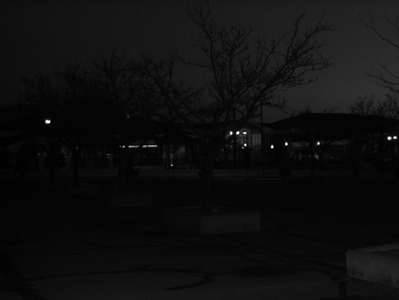
\includegraphics[width=\linewidth]{LC1.png}
        \caption{Given image, without any enhancements of any kind.}
        \label{lc1_orig}
    \end{subfigure}
    \begin{subfigure}{0.32\linewidth}
        \centering
        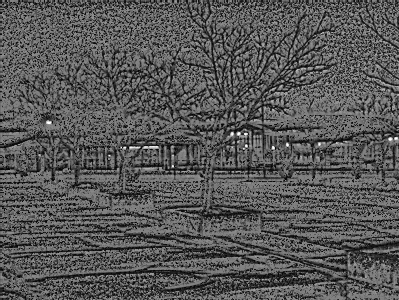
\includegraphics[width=\linewidth, keepaspectratio]{smol_enhanced_LC1.png}
        \caption{Image enhanced using Adaptive Histogram Equalization with $7\times 7$ blocks.}
    \end{subfigure}
    \begin{subfigure}{0.32\linewidth}
        \centering
        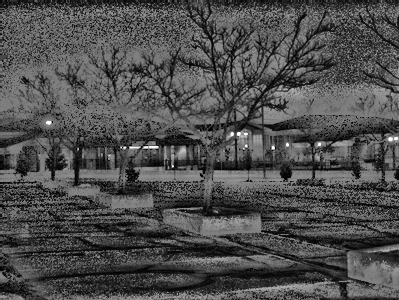
\includegraphics[width=\linewidth]{medium_enhanced_LC1.png}
        \caption{Image enhanced using Adaptive Histogram Equalization with $31\times 31$ blocks.}
    \end{subfigure}
\end{figure}
\begin{figure}
    \centering
    \begin{subfigure}{0.32\linewidth}
        \centering
        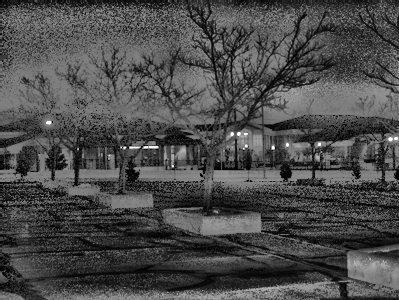
\includegraphics[width=\linewidth]{big_enhanced_LC1.png}
        \caption{Image enhanced using Adaptive Histogram Equalization with $51\times 51$ blocks.}
    \end{subfigure}
    \begin{subfigure}{0.32\linewidth}
        \centering
        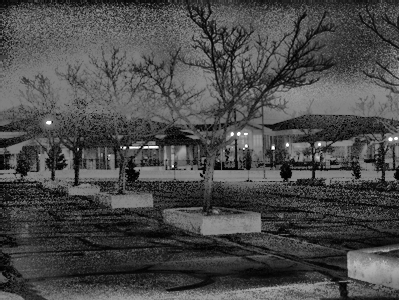
\includegraphics[width=\linewidth]{chonky_enhanced_LC1.png}
        \caption{Image enhanced using Adaptive Histogram Equalization with $71\times 71$ blocks.}
        \label{lc1_71_ahe}
    \end{subfigure}
    \begin{subfigure}{0.32\linewidth}
        \centering
        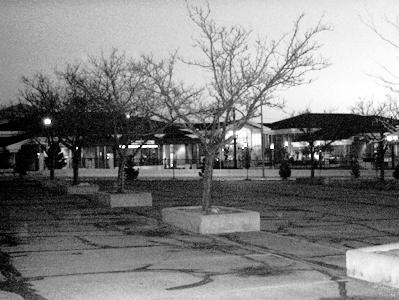
\includegraphics[width=\linewidth]{global_histogram_LC1.jpg}
        \caption{Image enhanced using Global Histogram Equalization.}
        \label{lc1_ghe}
    \end{subfigure}
\end{figure}

\begin{figure}
    \centering
    \begin{subfigure}{0.32\linewidth}
        \centering
        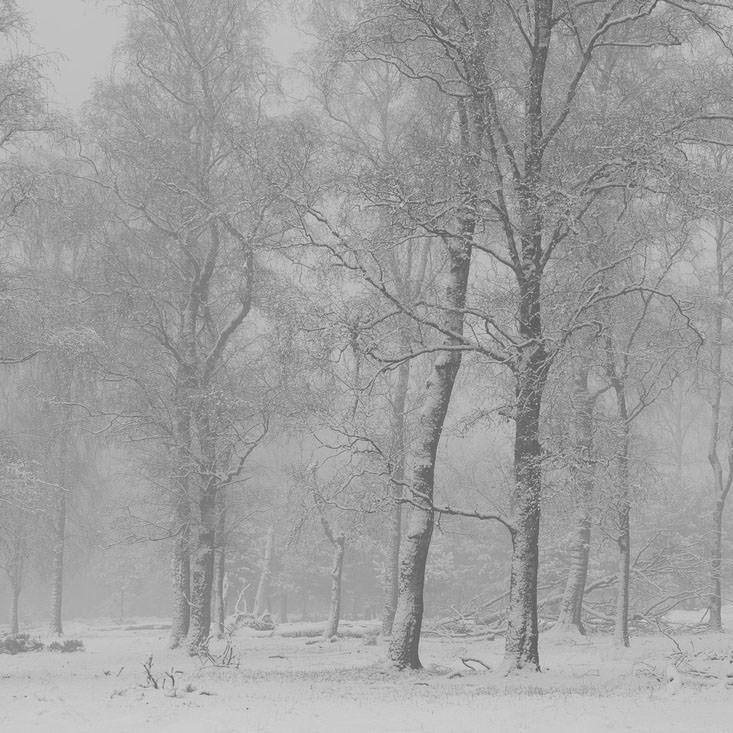
\includegraphics[height=0.4\textheight, keepaspectratio]{LC2.jpg}
        \caption{Given image, without any enhancements of any kind.}
        \label{lc2_orig}
    \end{subfigure}
    \begin{subfigure}{0.32\linewidth}
        \centering
        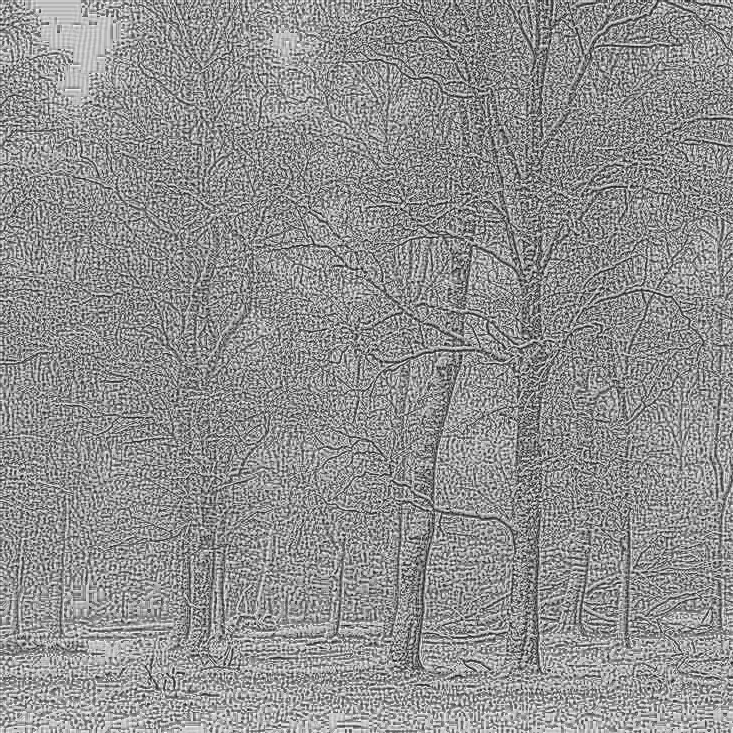
\includegraphics[height=0.4\textheight, keepaspectratio]{smol_enhanced_LC2.png}
        \caption{Image enhanced using Adaptive Histogram Equalization with $7\times 7$ blocks.}
    \end{subfigure}
    \begin{subfigure}{0.32\linewidth}
        \centering
        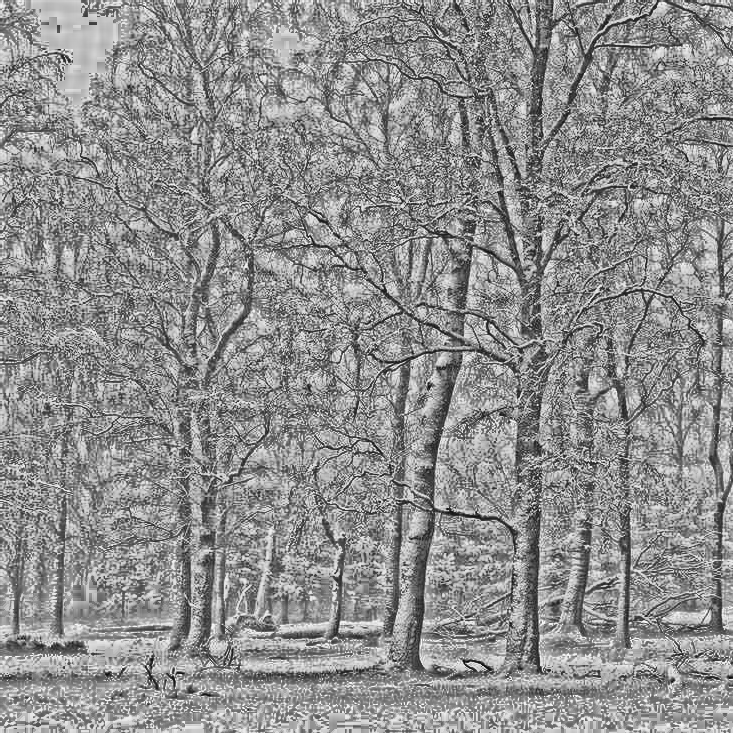
\includegraphics[height=0.4\textheight, keepaspectratio]{medium_enhanced_LC2.png}
        \caption{Image enhanced using Adaptive Histogram Equalization with $31\times 31$ blocks.}
    \end{subfigure}
\end{figure}
\begin{figure}
    \centering
    \begin{subfigure}{0.32\linewidth}
        \centering
        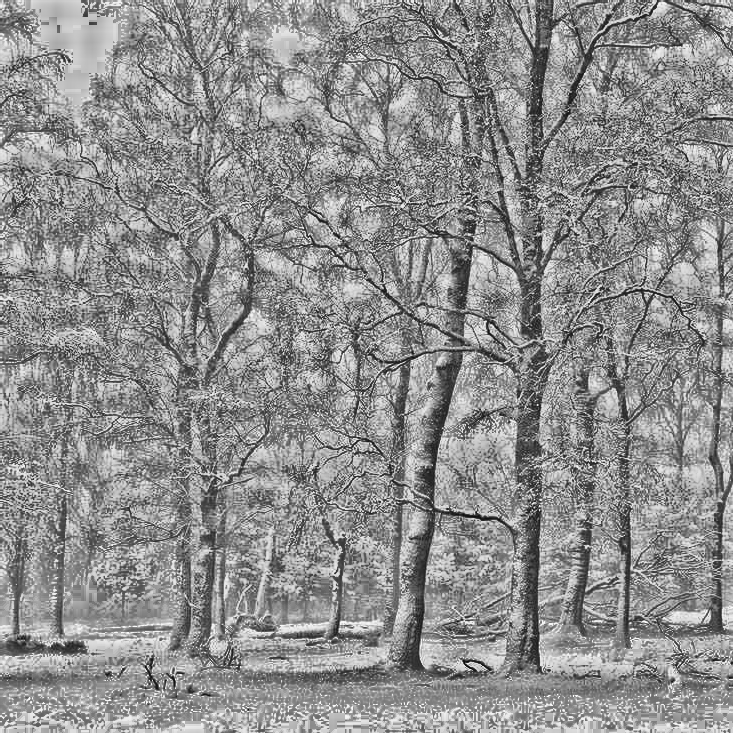
\includegraphics[height=0.4\textheight, keepaspectratio]{big_enhanced_LC2.png}
        \caption{Image enhanced using Adaptive Histogram Equalization with $51\times 51$ blocks.}
    \end{subfigure}
    \begin{subfigure}{0.32\linewidth}
        \centering
        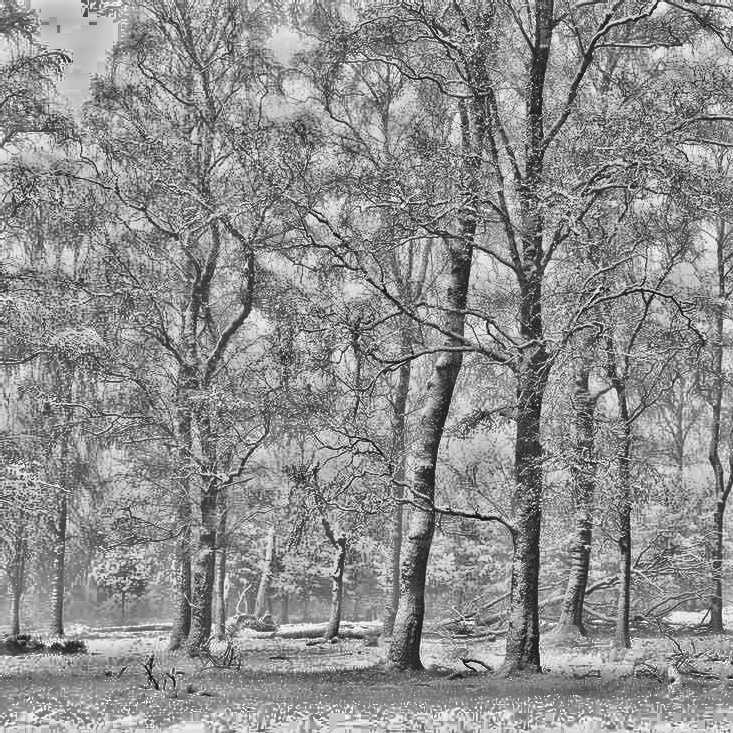
\includegraphics[height=0.4\textheight, keepaspectratio]{chonky_enhanced_LC2.png}
        \caption{Image enhanced using Adaptive Histogram Equalization with $71\times 71$ blocks.}
        \label{lc2_71_ahe}
    \end{subfigure}
    \begin{subfigure}{0.32\linewidth}
        \centering
        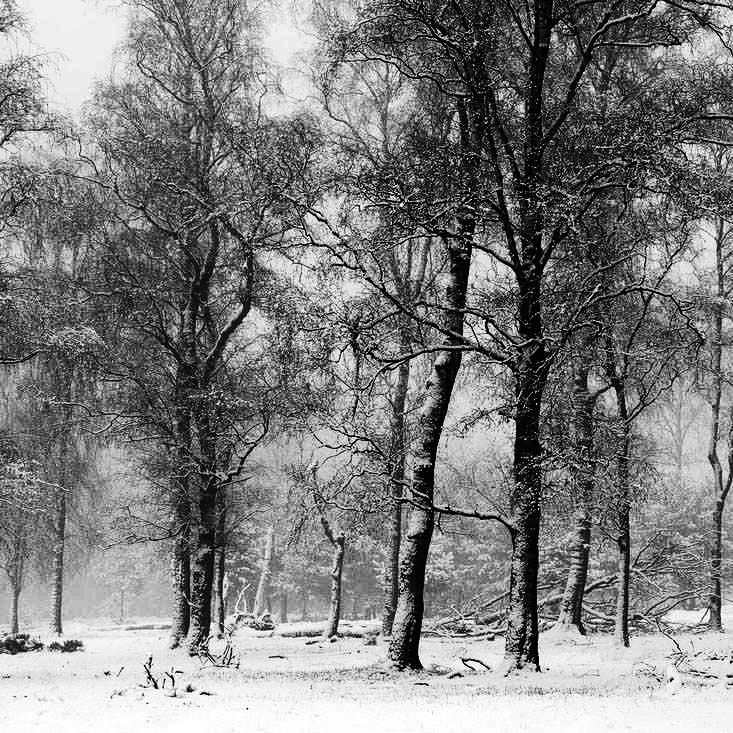
\includegraphics[height=0.4\textheight, keepaspectratio]{global_histogram_LC2.jpg}
		\caption{Image enhanced using Global Histogram Equalization.}
        \label{lc2_ghe}
    \end{subfigure}
\end{figure}
\end{document}